\subsection{Gradient descent}

\begin{frame}\frametitle{Finding the minumum of $\ETw$ iteratively}

\mode<article>{

Learning from gradient descent is an alternate approach for finding the minimum of a function when the closed-form solution is not available.

}
    \begin{figure}[h]
        \centering
        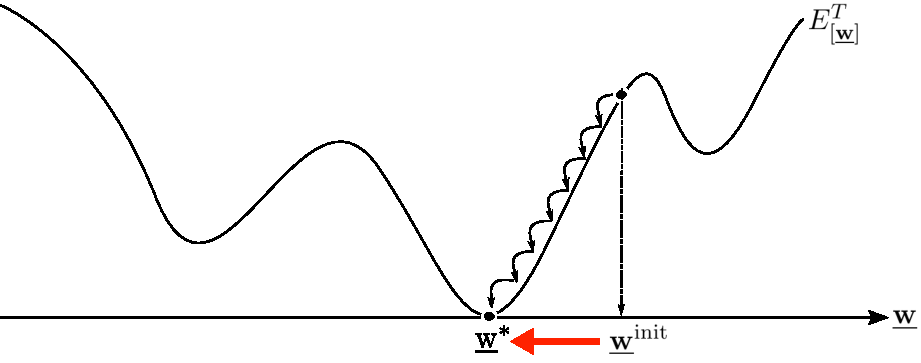
\includegraphics[height=3.cm]{img/section1_fig19}
        \notesonly{\caption{Minimizing the training error iteratively via gradient descent}
        }
        \label{fig:minimize_via_gradient_descent} 
    \end{figure}
    
    For our connectionist neuron example\notesonly{ learning by gradient descent would update each weight iteratively using}:
    \begin{equation}
    		w_{j}(t+1) \quad=\quad w_{j}(t) 
				\;\;{\color{red}-}\;\;
				\underbrace{{\eta}}_{ 
						\substack{\text{learning} \\ \text{step} } }
                        \cdot
				\underbrace{\frac{\partial \ETw}{
					\partial {w}_{j}}}_{
						\substack{
							\text{component of}\\
							\text{\textcolor{red}{gradient vector}} 
			} }
            \label{eq:gradient_descent_neuron}
    \end{equation}
    
    with $j=0,\ldots,N$
    \mode<article>{
    $\vec w^{\mathrm{init}}$ from \figref{fig:minimize_via_gradient_descent} is a random guess of where the solution might be and going against the gradient will potentially move us closer to the minimum. 
    }
    
    \mode<article>{
    
    The learning step (learning rate) $\eta$ modulates the magnitude of our update. $\eta$ can be treated as a constant but we will also see how the value of $\eta$ can change over time, i.e. $\eta(t)$.
    }
    \only<2>{
        \svspace{-2mm}
        \question{Why do we \underline{subtract} the gradient from $w_{j}(t)$?}
    }
    
    \mode<article>{
        The gradient describes the slope. Adding it will move us upwards and potentially maximize our function. Gradient-based learning with the intention of maximizing some function is referred to as hill climbing or gradient \emph{ascent}.
    }
    
    \only<3>{
    \question{So what is the downside of using gradient descent?}\\
    }
\end{frame}

\mode<article>{

    - The solution we find heavily depends on the initial position we started from. Indeed, gradient descent will reduce our cost each step but it does not guarantee that it will find the global minimum and will also stop at a local minimum. The slope in both cases is equal to zero.
    }

\begin{frame}\frametitle{\subsecname}
    
   \mode<presentation>{
    
    \textbf{So what's the downside of using gradient descent?}\\
    
    }
    
    \begin{figure}[h]
        \centering
        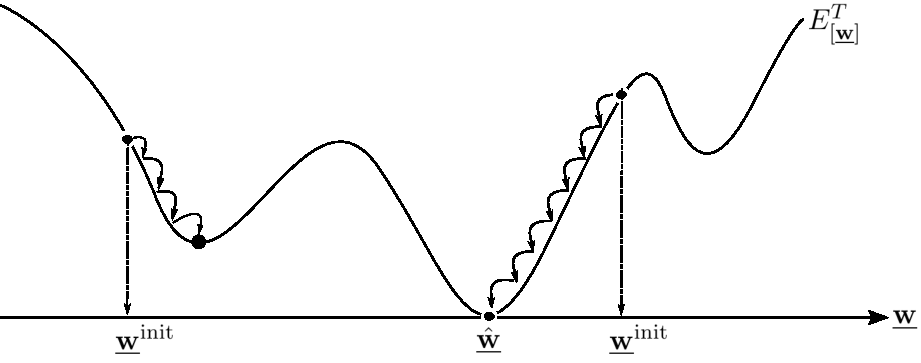
\includegraphics[height=3.25cm]{img/section1_fig19_local}
        \caption{Gradient descent finds local minima. We therefore denote the solution with $\hat{\vec w}$}
        \label{fig:minimize_via_gradient_descent_local} 
    \end{figure}
    
\end{frame}

\subsection{Gradient calculation: Connectionist neuron}

\begin{frame}\frametitle{Gradient calculation: Connectionist neuron}
    
    \begin{figure}[h]
        \centering
        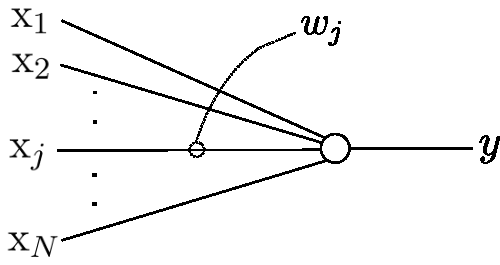
\includegraphics[height=\notesonly{1.9cm}\slidesonly{2.5cm}]{img/linearNeuron_y}
        \mode<article>{
        \caption{A connctionist neuron}
        }
        \label{fig:neuron} 
    \end{figure}
    
    \mode<presentation>{
    Working with the connectionist neuron\notesonly{ from figure \figref{fig:neuron}}, gradient descent updates the weights using:
    \begin{equation}
    		w_{j}(t+1) \quad=\quad w_{j}(t) 
				\;\;{\color{red}-}\;\;
				\underbrace{{\eta}}_{ 
						\substack{\text{learning} \\ \text{step} } }
                        \cdot
				\underbrace{\frac{\partial \ETw}{
					\partial {w}_{j}}}_{
						\substack{
							\text{component of}\\
							\text{\textcolor{red}{the gradient}} 
			} }
    \end{equation}
    }
    
\end{frame}
\begin{frame}
    
    \only<1>{
    Knowing that
    \begin{align}
		\frac{\partial \ETw}
			{\partial {w}_{j}}
		\;&=\; \frac{1}{p} \sum_{\alpha=1}^p
        \frac{\partial e\tyxwalpha}
			{\partial {w}_{j}}
        =\; \frac{1}{p} \sum_{\alpha=1}^p 
        \frac{\partial e^{(\alpha)}}
			{\partial {w}_{j}}
	\end{align}
    }
    with $j=0,\ldots,N$.\\
    
    \mode<article>{
    The individual cost $e^{(\alpha)}$ is a function of terms that are functions of other terms themselves. Therefore, $\frac{\partial e^{(\alpha)}}{\partial {w}_{j}}$ is computed by applying the \emph{chain rule}:\\
    }
    \only<1,2>{
	\begin{equation}
		\frac{\partial \ETw}
			{\partial {w}_{j}}
		\;=\; \frac{1}{p} \sum_{\alpha=1}^p	\underbrace{
			\textcolor{blue}{
			\frac{\partial e\tyxwalpha}{\partial 
					y(\vec{x}^{(\alpha)}, \vec{w})} }}_{
						\substack{\text{factor depending} \\
							\text{on cost function}}}
				  \;\cdot \underbrace{
			\textcolor{orange}{
			\frac{\partial y(\vec{x}^{(\alpha)}; \vec{w})}{
					\partial {w}_{j}}} }_{
						\substack{\text{factor depending on} \\
							\text{model class}\\
                            \text{(e.g. perceptron, MLP)}}}
            \label{eq:gradient_terms}
	\end{equation}
    }
    
    \mode<article>{
    The first factor
    represents the first link from applying the chain rule. One recognizes that it only depends on the choice of the cost function. This \emph{error term} is completely independent of the type of model we choose.\\
    }
    
    \only<1>{
    \notesonly{
    Therefore, if the objective were to minimize} quadratic error:
    
    \svspace{-1cm}
    \begin{equation}
			e\tyxw := \frac{1}{2} \left( y_T - y(\vec{x}; \vec w) \right)^2
    \end{equation}
    
    \mode<article>{it follows:}
    
    \begin{equation}
			\textcolor{blue}{\frac{\partial~e_{\text{quadr.}}\tyxwalpha}{
					\partial y{(\vec{x}^{(\alpha)}; \vec{w})} }
				= - y_T^{(\alpha)} + y{(\vec{x}^{(\alpha)}; \vec{w})}}
    \end{equation}
    }
    
\mode<article>{
    The model-specific contribution to the error appears in the \textcolor{orange}{second factor}.
    
    Continuing with our connectionist neuron \notesonly{from \figref{fig:neuron}}:
    }

    \mode<presentation>{\vspace{-5mm}}
    \only<2>{
    \begin{equation}
            y(\vec x; \vec w) := 
            f \Big(\; \sum_{j=0}^{N} {w}_{j} {x}_j
            \; \Big){}
            = f \left( \vec w^{\top} \vec x\right)
            = f \left( h (\vec x; \vec w)\right)
    \end{equation}
    
    It follows:
    \begin{align}
			\textcolor{orange}{
			\frac{\partial y(\vec{x}^{(\alpha)}; \vec{w})}
            {\partial {w}_{j}}}
            &= 
            \textcolor{magenta}{
            \frac{\partial y(\vec{x}^{(\alpha)}, \vec{w})}
            {\partial h(\vec x^{(\alpha)}; \vec w)}
            }
            \cdot
            \frac{\partial h(\vec x^{(\alpha)}; \vec w)}
            {\partial {w}_{j}}\\
            &= \underbrace{
            \textcolor{magenta}{
                f'(h(\vec x^{(\alpha)}; \vec w))
                }
            }_{\substack{\text{depends on}\\ \text{transfer function}}}
            \cdot
            \underbrace{
                \frac{\partial~\vec w^{\top} \vec x^{(\alpha)}}
                {\partial {w}_{j}}
            }_{=x_{j}}
	\end{align}
    }
    
\end{frame}

\mode<presentation>{
\begin{frame}
Again with less clutter:

	\begin{align}
		\frac{\partial \ETw}
			{\partial {w}_{j}}
		\;=\;& \frac{1}{p} \sum_{\alpha=1}^p	\underbrace{
			\textcolor{blue}{
			\frac{\partial e_{\text{quadr.}}\tyxwalpha}{\partial 
					y(\vec{x}^{(\alpha)}, \vec{w})} }}_{
						\substack{\text{factor depending} \\
							\text{on cost function}}}
				  \;\cdot \underbrace{
			\textcolor{orange}{
			\frac{\partial y(\vec{x}^{(\alpha)}; \vec{w})}{
					\partial {w}_{j}}} }_{
						\substack{\text{factor depending on} \\
							\text{model class}\\
                            \text{(e.g. perceptron, MLP)}}}\\
            \;=\;& \frac{1}{p} \sum_{\alpha=1}^p
            \textcolor{blue}{(y{(\vec{x}^{(\alpha)}; \vec{w}) - y_T^{(\alpha)})}}
            \cdot
            \textcolor{orange}{
            f'(h(\vec x^{(\alpha)}; \vec w))
            \cdot
            x_{j}
            }
	\end{align}

\begin{center}
	\includegraphics<2->[width=0.2\textwidth]{img/meme_perceptron_grad}
\end{center}

\end{frame}

\begin{frame}\frametitle{Computing gradients for an MLP}

Next time.
\end{frame}
}
